\chapter{Disassembler}
A disassembler is a computer program that translates machine language into assembly language-the inverse operation to that of an assembler. A disassembler differs from a decompiler, which targets a high-level language rather than an assembly language. Disassembly, the output of a disassembler, is often formatted for human-readability rather than suitability for input to an assembler, making it principally a \textbf{reverse-engineering tool}.

\section{Disassembler Demonstration}
\Cref{fig:s1asm} shows a sample program i.e. "\textit{1's COMPLEMENT OF A 16-BIT NUMBER}" loaded in the assembly language editor. It is then assembled by pressing the \textbf{Assemble} button. After assembling, memory content  and assembler workspace are shown in \cref{fig:s1asmMem} and \cref{fig:s1asmWork} respectively. Then the \textbf{Hexcode} is saved by selecting "FILE$ \rightarrow $Save Hexcode" or presing "ALT+S". \\

The generated hexcode is now loaded in the Disassembler editor by selecting "FILE$ \rightarrow $Load Hexcode" or presing "ALT+O". As it can be seen in \cref{fig:s1hex} the Intel Hex formatted code is syntactically highlighted.
Now, press the \textbf{Disassemble}. If there is some error in the code that line will be highlighted in red.  The tabbed window will not automatically change, even if there is no error. Now open the assembler editor the code is disassembled, as given in \cref{fig:s1dis}. Simultaneously the memory content is also loaded which is same as shown in \cref{fig:s1asmMem}. But, it is to be remembered that assembler workspace will remain empty, until the code is assembled from the assembler editor.  

\begin{figure}[htbp]
        \centering
        \begin{subfigure}[b]{0.4\textwidth}
                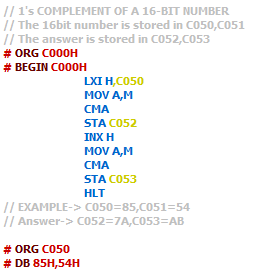
\includegraphics[width=\textwidth]{sampleCode1}
                \caption{Assembled Code}
                \label{fig:s1asm}
        \end{subfigure}
       \begin{subfigure}[b]{0.3\textwidth}
                       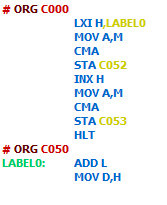
\includegraphics[width=\textwidth]{sampleCode1Rev}
                       \caption{Disassembled Code}
                       \label{fig:s1dis}
               \end{subfigure}
		\\        \vspace{20pt}
       \begin{subfigure}[b]{0.5\textwidth}
                       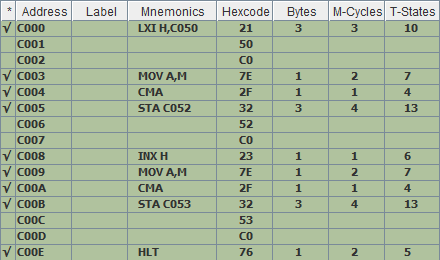
\includegraphics[width=\textwidth]{sampleCode1Asm}
                       \caption{Assembler Workspace after Assembling}
                       \label{fig:s1asmWork}
               \end{subfigure}
       \begin{subfigure}[b]{0.4\textwidth}
                       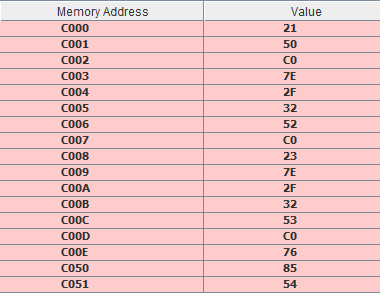
\includegraphics[width=\textwidth]{sampleCode1Mem}
                       \caption{Memory Content after Assembling}
                       \label{fig:s1asmMem}
               \end{subfigure}    
		\\        \vspace{20pt}
       \begin{subfigure}[b]{0.5\textwidth}
                       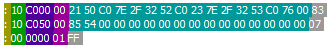
\includegraphics[width=\textwidth]{sampleCode1Hex}
                       \caption{Hexcode of Assembled code}
                       \label{fig:s1hex}
               \end{subfigure}    
         \\ \vspace{20pt}          
   \caption{Showing working of Disassembler}
\end{figure}
\section{Intel HEX}
Intel HEX\cite{hex}  is a file format for conveying binary information for programming 8085 microprocessor. The assembler converts the program's assembly language code to machine code and outputs it into a HEX file. That file is then imported by a programmer to "burn" the machine code to the 8085 target system for loading and execution.

\begin{figure}[H]
\centering
\includegraphics{"./disassemble"}
\begin{tabular}{cl}
{\color[HTML]{999900}\rule{0.5cm}{0.5cm}} & Start Code\\
{\color[HTML]{009900}\rule{0.5cm}{0.5cm}} & Byte count\\
{\color[HTML]{4C0099}\rule{0.5cm}{0.5cm}} & Address\\
{\color[HTML]{990099}\rule{0.5cm}{0.5cm}} & Record type\\
{\color[HTML]{009999}\rule{0.5cm}{0.5cm}} & Data\\
{\color[HTML]{999999}\rule{0.5cm}{0.5cm}} & Checksum
\end{tabular}

\caption[width=0.75\linewidth]{Intel HEX file format}
\label{fig:hex}
\end{figure}

Each line of Intel HEX fileconsists of six parts  :
\begin{itemize}
\item \textbf{Start code}, one character, an ASCII colon ':'.
\item \textbf{Byte count}, two hex digits, a number of bytes (hex digit pairs) in the data field. 16 (0x10) or 32 (0x20) bytes of data are the usual compromise values between line length and address overhead.
\item \textbf{Address}, four hex digits, a 16-bit address of the beginning of the memory position for the data.
\item \textbf{Record type}, two hex digits, 00 to 05, defining the type of the data field.
	\begin{itemize}
	\item \textbf{00}, data record, contains data and 16-bit address.
	\item \textbf{01}, End Of File record. Must occur exactly once per file in the last line of the file. The byte count is 00 and the data field is empty. Usually the address field is also 0000, in which case the complete line is ':00000001FF'.
	\end{itemize}
\item \textbf{Data}, a sequence of n bytes of the data themselves, represented by 2n hex digits.
\item \textbf{Checksum}, two hex digits - the least significant byte of the two's complement of the sum of the values of all fields except fields 1 and 6 (Start code ":" byte and two hex digits of the Checksum). It is calculated by adding together the hex-encoded bytes (hex digit pairs), then leaving only the least significant byte of the result, and making a 2's complement (either by subtracting the byte from 0x100, or inverting it by XOR-ing with 0xFF and adding 0x01). If you are not working with 8-bit variables, you must suppress the overflow by AND-ing the result with 0xFF. The overflow may occur since both 0x100-0 and (0x00 XOR 0xFF)+1 equal 0x100. If the checksum is correctly calculated, adding all the bytes (the Byte count, both bytes in Address, the Record type, each Data byte and the Checksum) together will always result in a value wherein the least significant byte is zero (0x00).
\\For example, on :0300300002337A1E\\
03 + 00 + 30 + 00 + 02 + 33 + 7A = E2, 2's complement is 1E
\end{itemize}


\section{Writing Hexcode in Disassembler}
\begin{itemize}


\item \textbf{STEP 1:} To Enter the hexcode\\

\begin{tabular}{cccccc}
\textbf{<Start Code>} & \textbf{<Byte Count>} & \textbf{<Address>} & <\textbf{Record Type>} & \textbf{<Data>} & \textbf{<Checksum>}\\
: & 10 & 0000 & 00 & Enter 10 bytes  & <ctrl+space>\\
&&&& of data in Hexadecimal&\\
&&&& format &
\end{tabular}

\item \textbf{STEP 2:} To mark end of file\\

\begin{tabular}{cccccc}
\textbf{<Start Code>} & \textbf{<Byte Count>} & \textbf{<Address>} & <\textbf{Record Type>} & \textbf{<Data>} & \textbf{<Checksum>}\\
: & 00 & 0000 & 01 &  & FF
\end{tabular}

\end{itemize}

\paragraph{TOOLS EMBEDDED IN DISASSEMBLER EDITOR}
\begin{itemize}
\item \textbf{\textit{AUTO CHECKSUM GENERATION}} \\ Just press \textbf{CTRL+SPACE} at the end of each line it is auto calculated and appended to that line
\item \textbf{\textit{AUTO SYNTAX HIGHLIGHTING and FORMATING}} \\It is activated on pressing of \textbf{ENTER} key.  
\end{itemize}

\subsection{Limitation of disassembler}
\begin{itemize}
\item Cannot determine the begin address of execution
\item Fails to distinguish between user defined data code and opcode, so it by default decode all as opcode.
\end{itemize} 